\documentclass{article}
%\usepackage{authblk}

\usepackage{graphicx}
\usepackage{float}
%\usepackage{fullpage}
\usepackage[utf8]{inputenc}
\usepackage{hyperref}

\usepackage[spanish]{babel}
\usepackage{amssymb,amsmath}
\usepackage{caption}
\captionsetup[figure]{font=scriptsize,labelfont=scriptsize}
\decimalpoint

%\usepackage[backend=bibtex,
%style=authoryear
%style=alphabetic
%style=reading
%]{biblatex}
%\addbibresource{bib}

\usepackage{xcolor}


\title{Algoritmos de deformación de mallas poligonales para sistemas de 
procesamiento digital de geometría}

\author{Plan de Tesis\\
        Director: Gabriel Taubin\\
        Co-director: Fernando Cukierman\\
        Consejero de estudios: Agustín Gravano\\
        Estudiante: Manuel Dubinsky}


\begin{document}


% Doctorado UBA: Artículo 10º. El tema y Plan de Tesis deberán ser presentados a la Comisión de Doctorado para su consideración y eventual aprobación por el Consejo Directivo, con el consentimiento del Director de Trabajo de Investigación y Plan de Tesis propuesto y del codirector, si lo hubiere, y una explicación de éste/os acerca de los medios disponibles para ser realizado, indicando el lugar donde se llevará a cabo la investigación. El Trabajo de Tesis deberá ser inédito y original. La publicación parcial de sus resultados con la aprobación del Director de Trabajo de Investigación y Plan de Tesis no invalidará el carácter de inédito requerido.

% Doctorado exactas: ARTICULO 14.-
% 14.1. Dentro de los dos (2) años de la aprobación del examen de admisión el Director de Tesis presentará el Plan de Tesis para su consideración a la Comisión de Doctorado, conjuntamente con el Doctorando. El mismo deberá contener la siguiente información:
% a- El tema de investigación sobre el cual versará el trabajo de Tesis.
% b- Lugar de trabajo.
% c- Antecedentes existentes sobre el tema.
% d- Naturaleza del aporte original proyectado.
% e- Disponibilidad de infraestructura y factibilidad de desarrollo del trabajo y su financiamiento.
% f - Plan de Trabajo.

\maketitle

%\begin{abstract}
%TODO
%\end{abstract}

%\tableofcontents

%\newpage

\section{Tema de investigación}
En los últimos años se ha producido una revolución técnica que generó un 
crecimiento sin precedentes en la capacidad de procesamiento de datos de 
los dispositivos de uso personal (ej.: notebooks y teléfonos celulares). 
En sintonía con esos cambios, el paradigma global en torno a la creación de 
software libre ha puesto a disposición herramientas sofisticadas de 
excelente calidad. En particular han surgido muchas herramientas de diseño 
para la industria, la arquitectura y el urbanismo, la exploración geográfica y 
el entretenimiento (ej.: cine de animación y juegos). Por otro 
lado, actualmente es posible producir modelos digitales 
tridimensionales muy precisos tomados de la realidad en base a diversas 
técnicas: resonancia magnética, tomografía computarizada, láser, 
ultrasonido, radarización, microscopía, etc. A las cuales se suman técnicas 
más económicas basadas en procesamiento de imágenes. 
Por último, hoy en día es posible producir objetos tridimensionales de 
buena calidad y bajo costo en base a técnicas de impresión 3D. La conjunción 
de estos tres hechos en relación al modelado tridimensional: (1) sistemas de 
captura de datos, (2) software de procesamiento e (3) impresión 3D, están determinando 
cambios drásticos en la producción de bienes y servicios.

% buscar alguna referencia de digital fabrication
\

El área de Procesamiento Digital de Geometría es la rama de la Ciencia 
de la Computación encargada de elaborar los modelos y algoritmos para 
analizar y manipular la información geométrica de los objetos 
tridimensionales. Más precisamente, provee herramientas para: reconstruir 
superficies a partir de conjuntos de puntos, filtrar el ruido en las 
muestras de puntos y manipular las formas (ej.: simplificarlas, deformarlas,
 suavizarlas y parametrizarlas) \cite{BKPAL:2010}. Se encarga además de 
 formular las estructuras de datos para modelar la información geométrica. 
 En este sentido, las mallas poligonales son las representaciones discretas 
 de los  objetos. Básicamente son grafos \cite{Harari:1969} que modelan, 
 superficies inmersas en el espacio tridimensional. Sus vértices son  
 una muestra de los puntos de la superficie. A cada vértice de la 
 malla se le asocia su posición en el espacio (ej.: coordenadas cartesianas). 
 Los ciclos simples del grafo se denominan “caras”. Las caras son polígonos 
 convexos simples (en general triángulos o cuadrados) que modelan una pequeña 
 parte de la superficie aproximando linealmente sus puntos interiores.

\

El contexto de nuestro trabajo es el problema de \emph{deformación de mallas 
poligonales}. Específicamente, una deformación $d: S \rightarrow S'$ es un 
mapa de una superficie $S$ en otra $S'$ que asocia a cada punto $p \in S$ 
un vector de desplazamiento $d(p)$, de este modo la superficie $S$ es 
deformada en la superficie $S'$:

$$S' := \{p + d(p) \ | \ p \in S\}$$

Para una representación de la superficie en términos de una malla poligonal, 
una deformación está completamente determinada por los vectores de desplazamiento 
$d_i = d(p_i)$ de los vértices de la malla $p_i \in S$. De modo que los 
desplazamientos de los puntos interiores de las caras se aproximan linealmente. \\
En la práctica, este problema debe ser considerado en el contexto de enriquecer 
la funcionalidad de las herramientas de diseño tridimensional. Es decir, por 
un lado hay que proveerle a los usuarios una interface simple para definir 
deformaciones de las superficies y por el otro, los algoritmos deben ser eficientes 
para brindar una respuesta interactiva. Típicamente la interface con los 
usuarios consiste en permitirles definir dos regiones sobre la superficie: 
(1) una región $H$ denominada \emph{manija} y una transformación afín (desplazamiento 
y/o rotación) de $H$ y (2) una región fija $F$ que permanecerá invariante. 
El algoritmo de deformación se encargará de producir una transformación 
suave del conjunto de puntos intermedios entre $F$ y $H$ (figura \ref{fig:def}). 
Denotaremos a dicho conjunto de puntos intermedios como el conjunto $R$. 

\

Nuestro trabajo consiste en diseñar e implementar nuevos algoritmos de 
deformación de superficies que resulten prácticos para las herramientas 
de diseño e impresión 3D.

\begin{figure}
	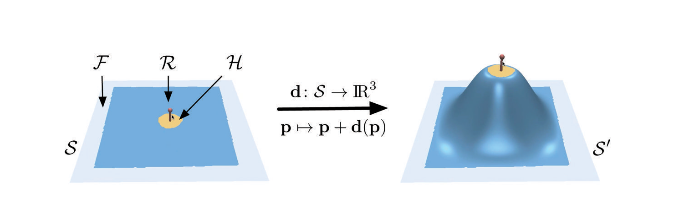
\includegraphics[scale=.5]{deformacion.png} % Figure image
	\caption{Una deformación $d: S \rightarrow S'$. Se define la manija 
	$H$ (región amarilla) y se desplaza verticalmente. La región 
	fija $F$ (gris) permanece invariante. La región $R$ (azul) entre $F$ 
	y $H$ se deforma suavemente.}% Figure caption
	\label{fig:def} % Label for referencing with \ref{bear}
\end{figure}

\section{Antecedentes existentes sobre el tema}

En la última década se produjeron varios trabajos en relación al problema 
de deformación de mallas poligonales. Esencialmente hay dos grandes enfoques 
para abordarlo: (1) deformaciones intrínsecas de la superficie y (2) deformaciones 
del espacio. Por un lado, las deformaciones intrínsecas consideran que la 
función de desplazamientos $d: S \rightarrow \mathbb{R}^3$ se define sobre 
la superficie $S$ y se calcula a partir de su malla poligonal asociada. Los 
métodos derivados de este enfoque son muy flexibles porque las condiciones 
se definen sobre cada vértice de la malla. Esa definición local de las 
condiciones incrementa los grados de libertad de las deformaciones. El inconveniente 
que presentan estas técnicas es que su eficiencia y robustez está asociada 
a la complejidad de la superficie y a la calidad de la muestra de puntos 
que conforman la malla poligonal. Por otro lado, el enfoque mediante deformaciones 
del espacio, considera que la función de desplazamientos $d: \mathbb{R}^3 
\rightarrow \mathbb{R}^3$ aplica sobre el espacio ambiente en el que está 
inmersa la superficie. De modo tal que la superficie se deforma implícitamente 
de acuerdo a la deformación global del espacio que la contiene. \\
A continuación presentamos los métodos más conocidos de cada uno de los  
enfoques. Recordemos de la sección anterior los tres conjuntos que intervienen 
en una deformación: (1) el conjunto $H$ (manija), (2) el conjunto $F$ (conjunto 
fijo o invariante) y (3) el conjunto $R$ (conjunto de puntos intermedios, 
o sea el soporte de la deformación).

\subsection{Métodos de deformaciones intrínsecas de la superficie}
Dentro de este enfoque, las técnicas más simples consisten en 
propagar la transformación afín de la manija ($H$) al conjunto 
$R$. Para que la transformación resulte suave entre $H$ y $F$, la propagación 
es controlada mediante una función de distancia $s: R \rightarrow [0,1]$ 
de cada punto de $R$ al conjunto fijo ($F$). Dicha función permite controlar 
para cada punto la magnitud de la transformación, de modo tal que los puntos 
cercanos a $H$ se transformen más que los puntos cercanos a $F$.


\subsection{Métodos de deformaciones del espacio}

\subsection{Otros temas relacionados}


\section{Naturaleza del aporte original proyectado}

Los resultados obtenidos a partir de este proyecto de investigación serán de gran valor para la comunidad que investiga y desarrolla en SDS y asistentes virtuales, así como también a la comunidad científica orientada a estudiar cómo los humanos interactuamos entre nosotros y con computadoras. Es así que, por un lado, los aportes serán en primer lugar importantes para generar nuevas hipótesis en torno a cómo los humanos interactuamos cuando dialogamos (tanto entre humanos como con computadoras) y a validar experimentalmente hipótesis previamente disponibles en la literatura o generadas por nosotros. Nótese que, aun cuando estos aportes sean netamente académicos y científicos, es de esperar que, sobre la base de los resultados que obtengamos, se puedan también extraer recomendaciones en torno a cómo mejorar los sistemas de diálogo que actualmente se encuentran incorporados tanto en computadoras personales como en dispositivos móviles. Debe mencionarse que existen concretos de este recorrido de la academia a la industria en el desarrollo de SDS, por ejemplo, en en el caso de toma de turnos en diálogo (\textit{turn-taking}).


\section{Lugar de trabajo, infraestructura, factibilidad de desarrollo del trabajo y su financiamiento}

El lugar de trabajo en el que se desarrollará mi doctorado es el Departamento de Computación (DC) de la Facultad de Ciencias Exactas y Naturales de la Universidad de Buenos Aires. El DC cuenta con un cluster de cómputo, diversos laboratorios de computación (que pueden ser utilizados para realizar experimentos), servicio de red, mail, web y hosting de servidores para grupos de investigación. Esta infraestructura comprende todo lo necesario para el desarrollo de mi propuesta de trabajo.

Desde el año 2015, formo parte del grupo de investigación LIAA (Laboratorio de Inteligencia Artificial Aplicada). El LIAA es un espacio interdisciplinario donde se emplean técnicas de inteligencia artificial y aprendizaje automático en diferentes problemáticas aplicadas. A este grupo pertenecen cuatro investigadores (incluyendo al director de mi doctorado), junto con estudiantes postdoctorado, doctorado y tesistas de licenciatura. Es de esperar que éstos no sólo guien mi trabajo, sino que sean colaboradores en distintos proyectos en los cuales participe. Por otra parte, el grupo me provee de computadora de escritorio, grabadores para habla, y una sala experimentale para poder trabajar. Finalmente, en  el DC se dictan numerosas materias de posgrado útiles para mi doctorado.

En lo referido a mi financiamiento, cuento con una beca de estudios proveniente de un convenio firmado, a través de la Fundación Ciencias Exactas, entre la Universidad de Buenos Aires y la Constantine the Philosopher University en Nitra, Eslovaquia. Adicionalmente, soy profesor titular de dos materias de grado dictadas en la Lic. en Economía Empresarial de la Universidad Torcuato di Tella.


\section{Plan de trabajo}

\begin{itemize}

\item Generación de nuevos estudios de corpus y análisis de corpus ya disponibles en nuestro grupo.

\item Colaboración en proyectos del grupo de investigación, sea a través de colaboración con otros investigadores o estudiantes de doctorado, o dirigiendo a tesistas de licenciatura del grupo.

\item Revisión del estado del arte en lo referido a la medición de atributos prosódicos y a la síntesis de los mismos.

\item Refinamiento de hipótesis, diseño experimental y ejecución de experimentos para validar hipótesis pre-existentes.

\item Publicación de resultados en conferencias y revistas de alto impacto.

\end{itemize}

\subsection{Avances ya realizados}

Hasta el momento hemos avanzado tanto en la línea de análisis de corpus como en la de diseño, ejecución y análisis de experimentos. En los referido a estudio de corpus, llevamos adelante un estudio orientado a analizar cómo se relacionan medidas de mimetización con aspectos sociales en conversaciones entre humanos (dicho estudio fue presentado en Interspeech 2016, \cite{perez2016disentrainment}). También hemos avanzado en tres experimentos de laboratorio. En el primero analizamos cómo impactan distintos esquemas de variaciones prośodicas en la selección de ayudantes virtuales (dicho estudio fue presentado en Interspeech 2016, \cite{levitan2016implementing}). En el segundo estudiamos cómo distintos atributos prosódicos impactan en el tiempo de respuesta asociado a responder si una declaración sintetizada es verdadera o no (dicho estudio fue enviado a Interspeech 2017 y actualmente se encuentra en etapa de evaluación). En el tercero, el cual se encuentra en etapa de diseño y implementación, evaluaremos cómo la mimetización a nivel de acto de diálogo (e.g., a nivel de preguntas o a nivel de respuestas) impacta en la confianza de los usuarios.

Con respecto a materias, hasta el momento logré la aprobación de las siguientes materias relacionadas con mi tema de doctorado.

\hfill

\centering
\begin{tabular}{l c c c}

\textsf{Materia} & \textsf{Período} & \textsf{Calificación} & \textsf{Puntaje}\\
\hline
Introducción a las Tecnologías del Habla & 2do 2012 & 9 & 3\\
Reconocimiento de Patrones & 1ro 2015 & 10 & 4\\
Introducción a la Neurociencia Computacional & 2do 2015 & 10  & 5 \\
Maestría en Data Mining & 1ro 2015 & -  & 5 \\ 
\hline
\end{tabular}

\bibliographystyle{plain}
\bibliography{bibliography}

\end{document}
